% last updated in April 2002 by Antje Endemann
% Based on CVPR 07 and LNCS, with modifications by DAF, AZ and elle, 2008 and AA, 2010, and CC, 2011; TT, 2014; AAS, 2016

\documentclass[runningheads]{llncs}
\usepackage{graphicx}
\usepackage{amsmath,amssymb} % define this before the line numbering.
\usepackage{ruler}
\usepackage{color}
\usepackage[width=122mm,left=12mm,paperwidth=146mm,height=193mm,top=12mm,paperheight=217mm]{geometry}
\usepackage{url}
\usepackage{hyperref}
\usepackage{tabularx}

%\graphicspath{{../pdf/}{..\DD2424-Project\plots}}

\begin{document}
% \renewcommand\thelinenumber{\color[rgb]{0.2,0.5,0.8}\normalfont\sffamily\scriptsize\arabic{linenumber}\color[rgb]{0,0,0}}
% \renewcommand\makeLineNumber {\hss\thelinenumber\ \hspace{6mm} \rlap{\hskip\textwidth\ \hspace{6.5mm}\thelinenumber}}
% \linenumbers
\pagestyle{headings}
\mainmatter
\def\ECCV16SubNumber{***}
\title{Character-Level Text Classification with different RNN Architectures}
\author{
	Ching-an Wu {\tt cawu@kth.se} \\
    Rithika Harish Kumar {\tt rihk@kth.se} \\
	Mathilda Strandberg von Schantz {\tt matvs@kth.se} \\
}
\institute{KTH Royal Institute of Technology}

\maketitle

%The final report should include the following sections:

\begin{abstract}
% • Abstract: Where you give an overview of the task and the findings
% of your work in a nutshell.

A character-level RNN is used to classify text(words) to the respective categories using Pytorch. This is an extension of a tutorial \cite{tutorial}. The extensions done to the tutorial include Long short term memory and Gated recurrent unit layers, as well as using a different dataset.   

\dots
\keywords{Character-Level, Text classification, RNN, LSTM, GRU, Pytorch}

\end{abstract}


\section{Introduction}

% • Introduction/Problem formulation: Motivate the problem you
% are trying to solve, attempt to make an intuitive description of the
% problem and also formally define the problem. (1-2 pages including
% title, authors and abstract)

We are looking at a text classification problem with short text and character-level classification. The data set used was initially the world-cities data set \cite{world-cities}, but was later extended to the bigger geonames data set \cite{geonames}. More specifically, its the collection of (city, country) pairs from the most highly populated cities of the world. There are circa 240 categories (countries) in both data sets, but we will limit the number of categories so as not to make the categories too unevenly distributed (ie remove countries with too few cities in the data set).

We will be using character-level classification. This means that the network processes the input one character at a time. Each character results in an output consisting of the probabilities for each letter for the next character. If we have a 58-character alphabet, the hidden state will consist of the probability of each of those 58 characters for the next letter in the sequence. So for each character, one such prediction is produced, as well as a hidden state, which is fed into the next step.

Short-text classification is hard in that there is less information to go off with little to no grammar or syntax. Some applications of short-text classification include search queries and information retrieval, mapping a product name to its associated product, the classification of titles, questions, sentences, and short messages.

The inspiration for the project is a tutorial in which a recurrent network is used to classify names as belonging to certain nationalities \cite{tutorial}. To start with, the model of that tutorial is to be replicated, then additional architectures will be implemented and compared. Questions we ask ourselves include: would the model on the tutorial work on a different data set? To what degree would a deeper network help in this problem? Would an LSTM-layer in the recurrent network give better results? 

To measure the success of the text classification, we will look at the average f1-score and accuracy across all categories in the data set. Furthermore, we will visualize the results with a confusion matrix.


\section{Background}

% • Background: summarize a few notable approaches/papers tackling
% the same problem. The selection should cover different possible tech-
% niques that can be (have been) used for the same task with success.
% Also, it is good to mention other recognition/synthesis tasks that use
% the same deep learning technique as yours. (1-2 pages)

Recurrent Neural Networks (RNNs) have been mainly used in sequential input learning problems such as text classification, speech recognition, translation and image captioning. For this project, our main goal is to use three different neural network architectures to perform character-level text classification and compare their performance based on the same datasets. The three networks are a vanilla Recurrent Neural Network (RNN), Long Short Term Memory network (LSTM) and Gated Recurrent Unit network (GRU). In fact, the last two networks are the variants of a classical RNN. 

In the related works, we can find that character-level neural network models have several advantages in comparison to word-level models or even n-gram neural networks. In \cite{low2016character}, Low M. stated that character-based model can reduce the use of memory significantly because there is no need to create word embedding matrix\cite{kim2016character}. As for text prediction, he also indicated character-level models were found to be outperformed by word-level models in general. In \cite{zhang2015character}, Zhang et al. also believed that in most cases character-based models had better performance because characters constitute a necessary construct no matter how text was separated, and they can still learn even abnormal character combinations such as misspellings and emoticons existed in text.    

Considering other variants of recurrent neural networks, \cite{de2018character} had a good explanation for them. This paper states that generating and modeling dynamic sequences of discrete tokens is the core application of character-based recurrent neural networks. In other words, RNNs are designed to maintain a summary of the past sequence in their memory or by so-called "hidden state". More over, they also mentioned that some extensions of vanilla RNN such as LSTM and GRU are designed to help maintain long-term dependencies and to address the vanishing gradient problem. Perhaps that is why in our task LSTM and GRU are not outperformed by classic RNN significantly. 

Apart from using RNN-only models in text classification, \cite{liu2017character} proposed a network which is a combination of convolutional neural networks (CNN) and recurrent neural network (RNN). The reason that Liu introduced a CNN into their model is because short text is characterized of short length, sparse features and strong context dependency. And as we know, CNN has a good performance when it comes to feature extraction. This paper also mentioned that most of techniques based on words always suffer from abnormal character combinations.   

\section{Theory}

This section consists of the workings of RNN, LSTM and GRU. The basis of the information in this section is taken from \cite{colah}.
 
\subsection{RNN - Recurrent Neural Networks}

Traditional neural networks do not use reasoning based on the previous events to inform the later ones. To allow information to persist, RNNs were used. These are networks with loops.

\begin{figure}[h!]
\centering
        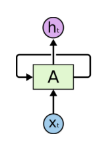
\includegraphics[width=0.2\linewidth]{plots/working_rnn}
    \caption{RNN Model}
\end{figure}

The above figure has a chunk of neural network A, with $x_t$ as input and $h_t$ as output. The loop allows information to be passed from one step to another. The basic equation is as follows:

\[state = W_x x_t + W_h h_{t-1} + b \]
\[h_t = tanh(state) \]

Although RNNs help in keeping the information, it is difficult to have long term dependencies. In practise, RNNs dont seem to learn it. So, LSTM came into play.

\subsection{LSTM - Long short term memory}

LSTM is a special kind of RNN which is capable of long-term dependencies. It is done by having a cell state. The cell state is kind of like a belt which allows information to just flow along it unchanged.
Cell states are regulated by three gates called forget($f_t$), input($i_t$) and output($o_t$). They help in optionally letting information through. Gates are composed of sigmoid neural net layer and pointwise multiplication operation.

\begin{figure}[h!]
\centering
        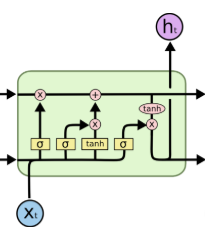
\includegraphics[width=0.4\linewidth]{plots/working_lstm}
    \caption{LSTM unit}
\end{figure}

First step is to decide what information to throw away from cell state. This is done by the sigmoid layer by outputting numbers between zero to one. Where zero means nothing is let through and one means everything is let through.

\[f_t = \sigma(W_f.[h_{t-1},x_t] + b_f) \]

Second step is to create a update. So decide what information to be stored in cell state. Next, a tanh layer creates a vector of candidate values($~C_t$) to be added.

\[i_t = \sigma(W_i.[h_{t-1},x_t] + b_i) \]
\[~C_t = tanh(W_c.[h_{t-1},x_t] + b_c) \]
\[C_t = f_t * C_{t-1} + i_t * ~C_t \]

Finally, we decide what parts of the cell to output by sigmoid layer. Then run a tanh and multiply with the output of sigmoid layer.

\[o_t = \sigma(W_o.[h_{t-1},x_t] + b_o) \]
\[ h_t = o_t * tanh(C_t)\]

This way LSTM has the ability to allow which information to pass through.
 
\subsection{GRU -  Gated Recurrent Unit}

The idea behind a GRU layer is quite similar to that of a LSTM layer except that GRU has only two gates. The input and forget gates are coupled by an update gate ($z_t$) and the reset gate ($r_t$) is applied directly to the previous hidden state.  

\begin{figure}[h!]
\centering
        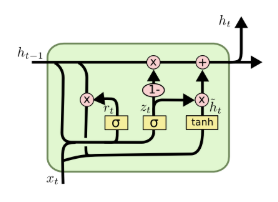
\includegraphics[width=0.5\linewidth]{plots/working_gru}
    \caption{GRU unit}
\end{figure}

\[z_t = \sigma(W_z.[h_{t-1},x_t]) \]
\[r_t = \sigma(W_r.[h_{t-1},x_t]) \]
\[~h_t = tanh(W.[r_t * h_{t-1},x_t]) \]
\[h_t = (1-z_t) * h_{t-1} + z_t * ~h_t \]

Intuitively, the reset gate determines how to combine the new input with the previous memory, and the update gate defines how much of the previous memory to keep around. If we set the reset to all 1’s and  update gate to all 0’s we again arrive at our plain RNN model.

\section{Approach}
% • Approach: Describe the final approach you are take for this problem.
% For instance, here you would describe the details of the network’s
% architecture. What training parameters and techniques you have used.
% The computational complexity of your model. And similar questions.
% To help explain your approach please make figures to accompany your
% text description. (1-3 pages)

\section{Experiments}

The first experiment was simply taking the model from the tutorial and running it on the first data set we had decided upon, the world-cities data set. 


\begin{figure}[h!]
	\centering
    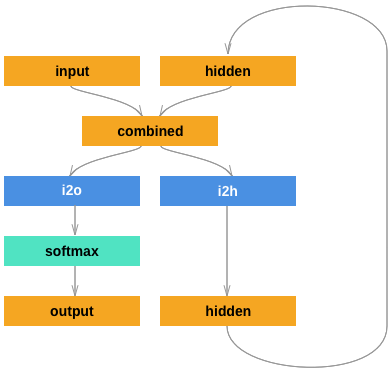
\includegraphics[width=.5\textwidth]{plots/tutorial_model.png}
	\caption{ Model from the text classification tutorial.}
	\label{fig:model_tutorial}
\end{figure}

The model in the tutorial is seen in figure \ref{fig:model_tutorial}, where i2o and i2h are simple linear layers that do a $y=Wx + b$ type calculation. Softmax is used to assign the different categories probabilities - it is a good way to represent a categorical distribution in a multi-class problem such as this one.
The criterion for loss that is used is negative log-likelihood loss.
The optimizer that is used is stochastic gradient descent. No momentum is used.
The \textit{combined} layer simply concatenates the input vector and hidden vector.

The data preprocessing was simple: the data was converted to ASCII-characters and the data was filtered to only have countries with at least 100 cities in the data set. This because the initial distribution was a bit too uneven, as seen in figure \ref{fig:world_cities}, with many countries having very few cities, some even just 1 or 2. What remained was 18684 data points.

\begin{figure}[h!]
	\centering
	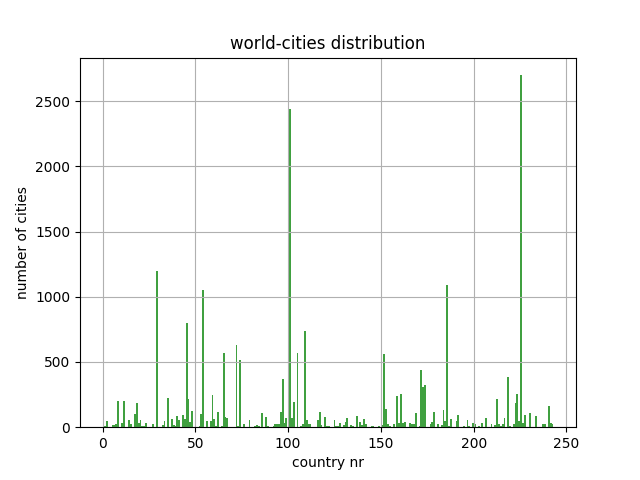
\includegraphics[width=.5\textwidth]{plots/dist.png}	
	\caption{ World-cities distribution.}
	\label{fig:world_cities}
\end{figure}

The training was done in a similar way as in the tutorial, with random sampling with replacement from the data set. The final confusion matrix looked is presented in figure \ref{fig:conf_init},
and the final average f1 score (averaged over all the categories) was 0.3. The test accuracy was 31 percent.

\begin{figure}[h!]
	\centering
        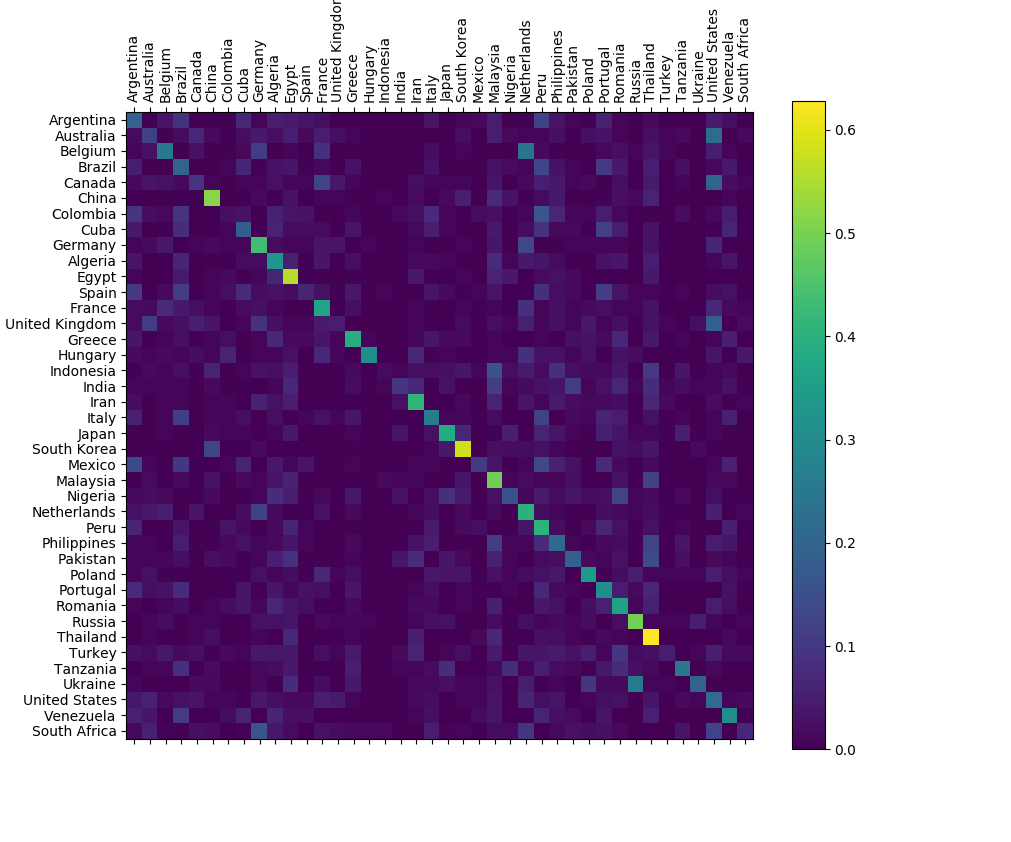
\includegraphics[width=.5\textwidth]{plots/confusion_matrix_initial.png}
	\caption{ Confusion matrix of first RNN model.}
	\label{fig:conf_init}
\end{figure}


While it is true that the model has a pretty good accuracy for some of the categories, it is still performing pretty unevenly for the categories. As seen in the figure, it is moderately good at classifying countries like Thailand and Korea, but not very good at classifying countries like Colombia or Indonesia (indeed it seems to never predict them). We do not see a clear pattern from the class distribution (for example the US is overrepresented in the data set but is not predicted more often than other countries). This is because of how the random sampling is made - first a random category is chosen, then a sample will be taken randomly from that category. Therefore, the number of times we're exposed to samples from different categories will be more or less even.

\subsection{Introducing LSTM and GRU}

We wanted to see if an LSTM-layer could improve the performance of the network. LSTMs are units used in recurrent networks that are composed of several gates - an input gate, output gate and forget gate. The LSTM can choose to "remember" or "forget" inputs from the past. This mechanism allows them to avoid the long-term dependency problem. However, this might not matter in this particular short-text classification problem, since there should not be long-term dependencies.

LSTMs are also supposed to be good against exploding and vanishing gradients, which is a common problem in backpropagation-through-time, the most common learning algorithm for standard recurrent networks.

The first LSTM experiment was simply running the same model as before, but replacing the linear layer for an LSTM layer.
 
\begin{figure}[h!]
	\centering
        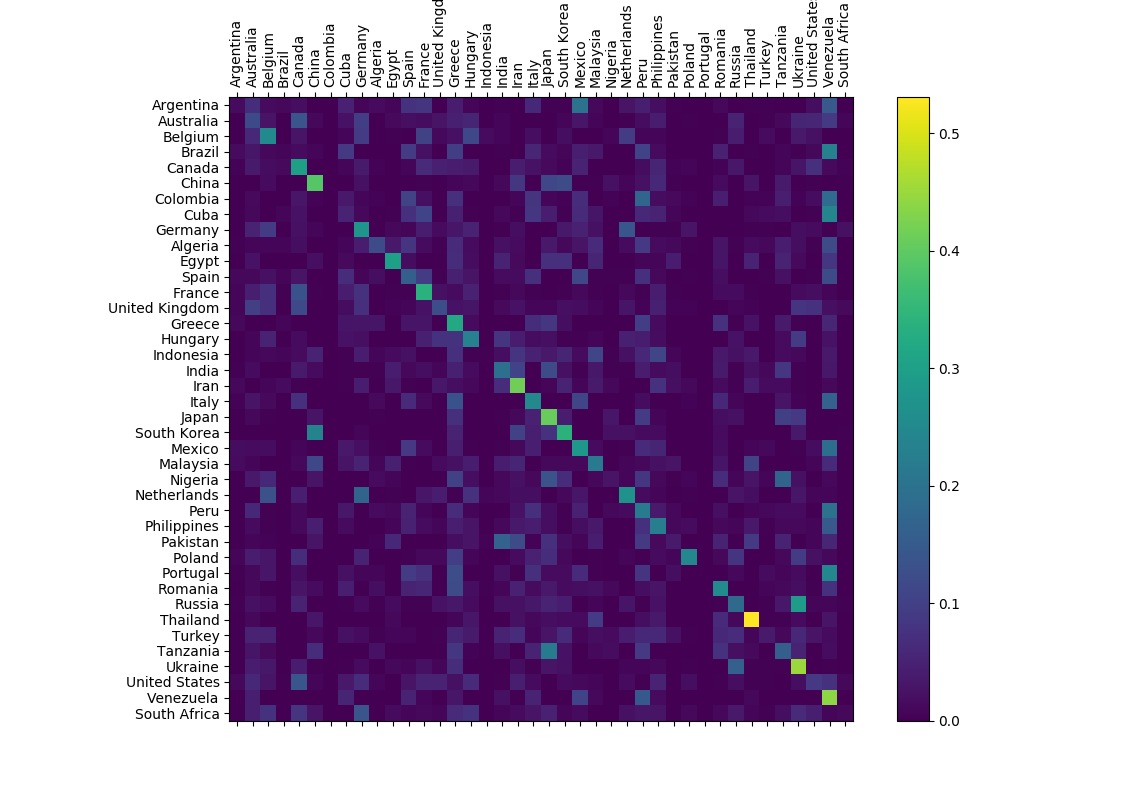
\includegraphics[width=.5\textwidth]{plots/conf_matrix_initial_LSTM.png}
	\caption{ Confusion matrix of first LSTM model.}
	\label{fig:conf_initial_lstm}
\end{figure}
 
It ended up not performing as well as the standard RNN after having been trained in the same way (same hyper-parameters, same number of epochs). As seen in figure \ref{fig:conf_initial_lstm}, the max accuracy is 0.5 rather than 0.6, and there are more incorrect predictions. Some more iterations of different LSTM architectures were tried. Things that were changed for each model are laid out in table \ref{tab:LSTMs}, and the results of the models are seen in table \ref{tab:LSTM_models}.

\begin{table}[h!]
    \begin{center}
        \caption{The changes introduced to different models.}
        \label{tab:LSTMs}
        \begin{tabularx}{.9\textwidth}{ | c | c | }
	        \hline
	        \textbf{LSTM model nr} & \textbf{difference introduced} \\ \hline
	        1 & introduced LSTM layer \\ \hline
	        2 & \begin{tabular}[x]{@{}c@{}} did combined input and \\ hidden (as in the original RNN)\end{tabular} \\ \hline
	        3 &  \begin{tabular}[x]{@{}c@{}} used a new data set called geonames,\\ that had more training samples\end{tabular} \\ \hline
	        4 & \begin{tabular}[x]{@{}c@{}} the previous model ran on all \\ countries in geonames that had more than 100 cities. \\ here the data was filtered more, and only \\ countries with more than 300 cities were used \end{tabular} \\ \hline
	        5 & tried not having class weights, to see if it actually helped \\ \hline
	        6 & used two LSTM layers \\ \hline
	        7 & \begin{tabular}[x]{@{}c@{}} instead of randomly sampling \\ with replacement, training consists of running \\ through the entire data set consisting of 81526 samples. \\ it was trained for 10 epochs \end{tabular} \\ \hline
	        8 & \begin{tabular}[x]{@{}c@{}} ran the model for 20 epochs. \\ checked validation error after every epoch. \\ also introduced shuffling of the data \\ before every epoch \end{tabular} \\ \hline
        \end{tabularx}      
        \end{center}
\end{table}
 

\begin{table}[h!]
    \begin{center}
        \caption{Results of the LSTM models.}
        \label{tab:LSTM_models}
        \begin{tabularx}{.5\textwidth}{ | c | c | c |}
			\textbf{model nr} & \textbf{average f1} & \textbf{test accuracy} \\
			1 & 0.18 & 21.6 \\
			2 & 0.2  & 21.9 \\
			3 & 0.04 & 7.5 \\
			4 & 0.14 & 17 \\
			5 & 0.2  & 17.2 \\
			6 & 0.1  & 12.8 \\
			7 & 0.23 & 27 \\
			8 & 0.3  & 38 \\
         \end{tabularx}  
    \end{center}
\end{table}

       
All LSTM models performed worse than the original RNN, up until model 8. Introducing the data set with more data points did not immediately lead to better results. This because there was an even bigger difference between classes (see figure \ref{fig:geonames}). 

\begin{figure}[h!]
	\centering
	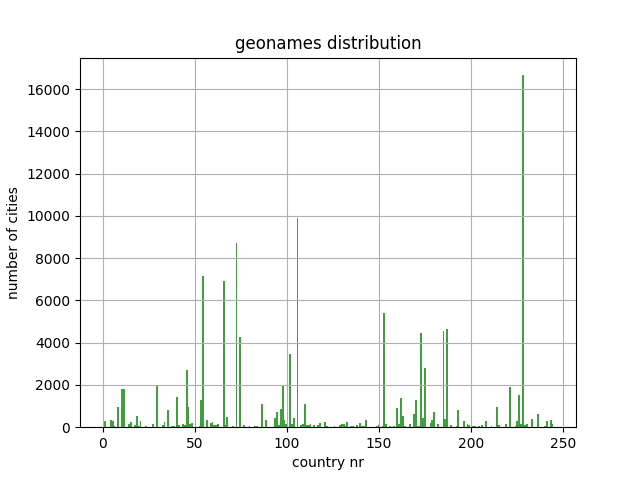
\includegraphics[width=.5\linewidth]{plots/geonames_set.png}
	\caption{ Geonames data set distribution.}
	\label{fig:geonames}
\end{figure}

This seemed to indicate that the data set needed to be filtered more, so all countries with less than 300 cities were removed.

After filtering the data more, the results were a bit better. However, the accuracy was still pretty low. Likewise, the model did not immediately perform better with two LSTM layers rather than one. It turns out that it simply needed to run for more epochs to account for the bigger data set and the bigger model. Indeed, model 8 performed best so far because it was run for more epochs.
 
After this, a GRU model was implemented and tested. It was run in the same way as LSTM model 8. And out of curiosity, a similar standard two-layer RNN was run in the same way. The result of this comparison is seen in table \ref{tab:GRU_LSTM_RNN_comp}.

\begin{table}[h!]
    \begin{center}
        \caption{Comparing the LSTM model with a similar model with GRU layers and one with linear layers.}
        \label{tab:GRU_LSTM_RNN_comp}
		\begin{tabularx}{.8\textwidth}{ | c | c | c |}
			\textbf{model description} & \textbf{average f1} & \textbf{test accuracy} \\
			LSTM model 8 & 0.3 & 38 \\
			similar GRU model & 0.32  & 42 \\
			similar standard RNN model & 0.09 & 12 \\
		\end{tabularx}  
    \end{center}
\end{table}

The GRU performed similar to the LSTM, just slightly better. However, it trained markedly faster. Meanwhile, the simpler RNN did not perform well, as it started suffering from exploding gradients. In its predictions, it exclusively predicted countries that are overrepresented in the data set. 

To look closer at the results of the GRU model, the confusion matrix is presented in figure \ref{fig:gru8}.  Note that this confusion matrix looks different from the previous, seeing as this is run on a different data set. The countries are here given by their two ISO 3166-1 codes. There are 55 categories in total, after having filtered the data. The confusion matrix is created by looking at 10 000 random samples taken from the test set.

\begin{figure}[!ht]
	\centering
	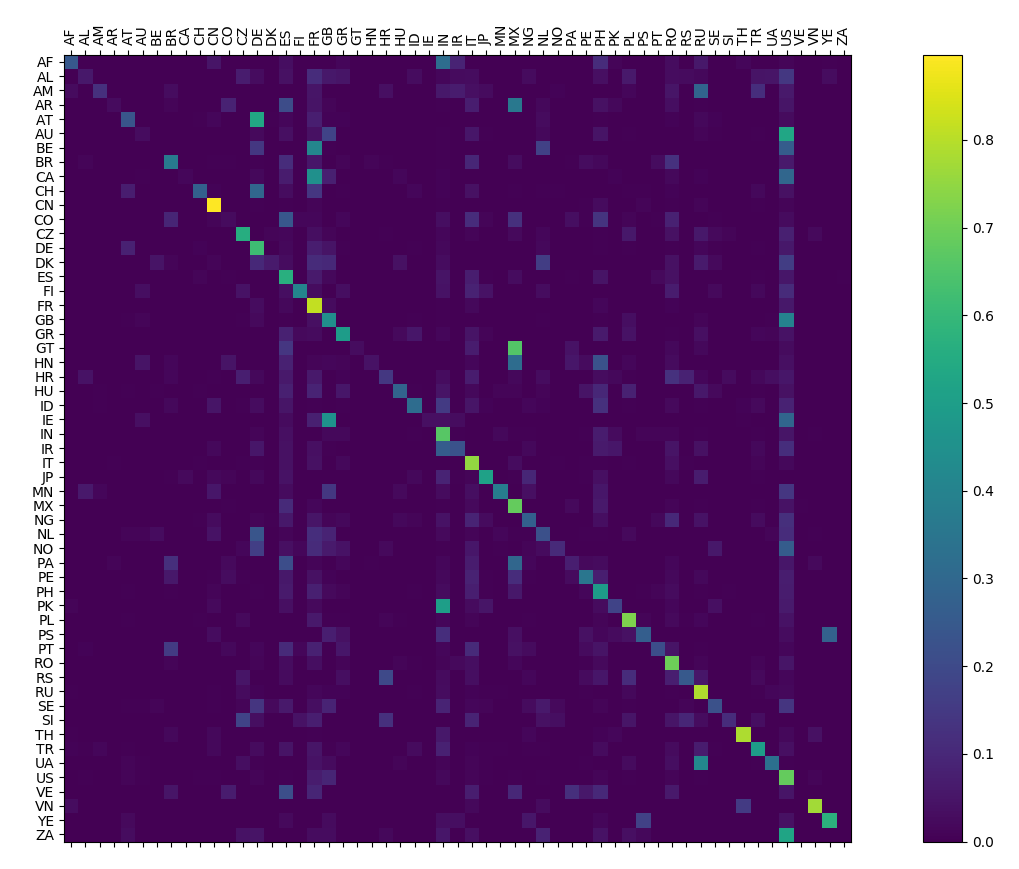
\includegraphics[width=.5\linewidth]{plots/conf_matrix_GRU_model_8.png}
	\caption{ Confusion matrix of the GRU model.}
	\label{fig:gru8}
\end{figure}

In the confusion matrix, we see that the model has a good accuracy on some countries. However, with so many categories it's hard to have a perfect prediction for all of them. Some countries are rarely predicted, while others are more likely to be predicted (such as the US and France). There are also some countries that are often confused with each other, such as (DE, AT), (GT,MX), (US,AU),(ZA,US), (PK, IN), and (UA, RU), which stand for the countries (Germany, Austria), (Guatemala, Mexico), (United States, Autralia), (South Africa, United States), (Pakistan, India), and (Ukraine, Russia). All of these seems sensible that the model would confuse, since they have similar languages and/or are close to each other geographically.

To see if the GRU model would perform better with more regularization, it was run in the same way as before but with a dropout of 20 percent. After that, it was explored whether that same model would perform better if trained with random sampling (ie ran for a number of epochs were, for each epoch, a training point is sampled randomly with replacement from the training set) yet again, but this time for more epochs. Perhaps running with random sampling is actually better for this application, since it would be less likely to overfit to overrepresented categories. Perhaps randomly sampling leads to better generalization in this instance.

Some more changes were introduced to the training of the model. One being that early stopping was introduced. The early stopping worked as follows: if the validation error has been increasing for \textit{patience} number of epochs, the model would stop training. \textit{patience} was set to 10. Furthermore, the model was only saved if the validation error was at its lowest. In this way, the model would not be saved when it started overfitting. The number of epochs was set to $1630520 = 81526 \cdot 20$, which is equivalent to running through the entire training set 20 times (since one "epoch" is just processing one randomly sampled training point).

The results of these experiments are given in table \ref{tab:additonal}.

\begin{table}[h!]
    \begin{center}
        \caption{Introducing dropout and training with random sampling again.}
        \label{tab:additonal}
		\begin{tabularx}{.8\textwidth}{ | c | c | c |}
			\textbf{model description} & \textbf{average f1} & \textbf{test accuracy} \\
			GRU with 0.2 dropout & 0.3 & 38 \\
			GRU with 0.2 dropout and random sampling & 0.39 & 48.5  \\
		\end{tabularx}  
    \end{center}
\end{table}

Only introducing dropout did not do much in terms of performance, while running with random sampling did perform better given more epochs to train. This because all countries receive a similar level of attention, which means the model might not have the highest maximum accuracy among all categories, but has a better average accuracy. This is also confirmed by the confusion matrix of the model given in figure \ref{fig:gru10}. This is the model that has performed most consistently good across all categories. While the number of epochs was set to 1 630 520 the model presented here was from when the validation error was at its lowest, which occurred on epoch 1 085 000.

\begin{figure}[!ht]
	\centering
	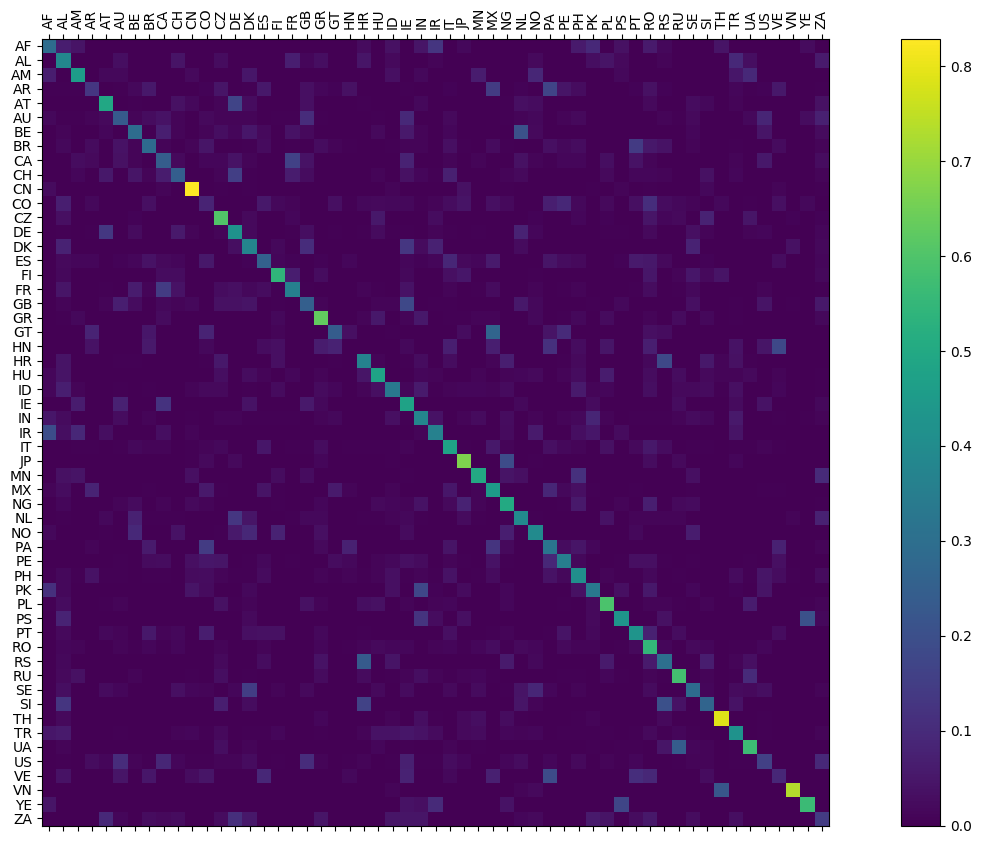
\includegraphics[width=.5\linewidth]{plots/conf_matrix_GRU_model_10.png}
	\caption{ Confusion matrix of the GRU model trained through random sampling from the data set.}
	\label{fig:gru10}
\end{figure}



%\section{Results} I think we should skip "Results" since all results are presented in the "Experiments" section //Mathilda

\section{Conclusions}

% • Experiments/Results/Conclusions: In this section, you should
% present the results you achieved with various experiments. The re-
% sults can be presented in tables, plots, etc. Explain what conclusions
% you can draw from these set of experiments? The set of experiments
% and results reported here should justify some of the design choices
% described in the previous sections. (3-6 pages)


% • References: It is extremely important to make sure all the content
% from other sources and the ideas that you build on are properly cited.


% Both positive and negative results should be reported. A discussion re-
% garding why certain techniques worked better than the others is necessary.
% Students are also encouraged to take initiatives in trying out new techniques,
% beyond those discussed at the lectures.
% The stated number of pages above is a guideline, one can go beyond that or
% slightly below. The whole report should be between 7-14 pages.

\clearpage

\bibliographystyle{splncs}
\bibliography{egbib}

\end{document}
